\documentclass[aspectratio=169]{beamer}
%\usepackage[english,greek]{babel}
%\usepackage[iso-8859-7]{inputenc}
\usepackage{euler}
\usepackage{tikz}

\beamertemplatenavigationsymbolsempty

\begin{document}
	\begin{frame}{$n=1$}
		\begin{figure}
			\centering
			\begin{tikzpicture}
			\draw[thick,->] (-.5,0) -- (4,0)node[pos=1,below]{$y$};
			\draw[thick,->] (0,-.5) -- (0,4)node[pos=1,left]{$x$};
			\node[below] at (pi,0){$\pi$};
			\draw[blue, thick, domain={0}:{pi}, samples=100] plot (\x,{\x^1*(pi-\x)^1/(1)});
			\end{tikzpicture}
		\end{figure}
	\end{frame}

	\begin{frame}{$n=2$}
		\begin{figure}
			\centering
			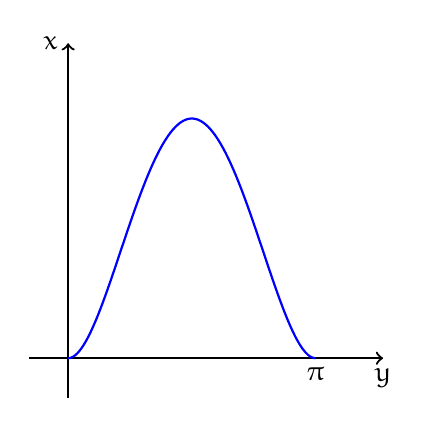
\begin{tikzpicture}
			\draw[thick,->] (-.5,0) -- (4,0)node[pos=1,below]{$y$};
			\draw[thick,->] (0,-.5) -- (0,4)node[pos=1,left]{$x$};
			\node[below] at (pi,0){$\pi$};
			\draw[blue, thick, domain={0}:{pi}, samples=100] plot (\x,{\x^2*(pi-\x)^2/(2)});
			\end{tikzpicture}
		\end{figure}
	\end{frame}

	\begin{frame}{$n=3$}
		\begin{figure}
			\centering
			\begin{tikzpicture}
			\draw[thick,->] (-.5,0) -- (4,0)node[pos=1,below]{$y$};
			\draw[thick,->] (0,-.5) -- (0,4)node[pos=1,left]{$x$};
			\node[below] at (pi,0){$\pi$};
			\draw[blue, thick, domain={0}:{pi}, samples=100] plot (\x,{\x^3*(pi-\x)^3/(6)});
			\end{tikzpicture}
		\end{figure}
	\end{frame}

	\begin{frame}{$n=4$}
		\begin{figure}
			\centering
			\begin{tikzpicture}
			\draw[thick,->] (-.5,0) -- (4,0)node[pos=1,below]{$y$};
			\draw[thick,->] (0,-.5) -- (0,4)node[pos=1,left]{$x$};
			\node[below] at (pi,0){$\pi$};
			\draw[blue, thick, domain={0}:{pi}, samples=100] plot (\x,{\x^4*(pi-\x)^4/(24)});
			\end{tikzpicture}
		\end{figure}
	\end{frame}

	\begin{frame}{$n=5$}
		\begin{figure}
			\centering
			\begin{tikzpicture}
			\draw[thick,->] (-.5,0) -- (4,0)node[pos=1,below]{$y$};
			\draw[thick,->] (0,-.5) -- (0,4)node[pos=1,left]{$x$};
			\node[below] at (pi,0){$\pi$};
			\draw[blue, thick, domain={0}:{pi}, samples=100] plot (\x,{\x^5*(pi-\x)^5/(120)});
			\end{tikzpicture}
		\end{figure}
	\end{frame}

	\begin{frame}{$n=6$}
		\begin{figure}
			\centering
			\begin{tikzpicture}
			\draw[thick,->] (-.5,0) -- (4,0)node[pos=1,below]{$y$};
			\draw[thick,->] (0,-.5) -- (0,4)node[pos=1,left]{$x$};
			\node[below] at (pi,0){$\pi$};
			\draw[blue, thick, domain={0}:{pi}, samples=100] plot (\x,{\x^6*(pi-\x)^6/(720)});
			\end{tikzpicture}
		\end{figure}
	\end{frame}

	\begin{frame}{$n=7$}
		\begin{figure}
			\centering
			\begin{tikzpicture}
			\draw[thick,->] (-.5,0) -- (4,0)node[pos=1,below]{$y$};
			\draw[thick,->] (0,-.5) -- (0,4)node[pos=1,left]{$x$};
			\node[below] at (pi,0){$\pi$};
			\draw[blue, thick, domain={0}:{pi}, samples=100] plot (\x,{\x^7*(pi-\x)^7/(7*720)});
			\end{tikzpicture}
		\end{figure}
	\end{frame}
\end{document}